% This work may be distributed and/or modified under the
% conditions of the LaTeX Project Public License version 1.3c,
% available at http://www.latex-project.org/lppl/.


\documentclass[10pt,a4paper,sans]{moderncv}        % possible options include font size ('10pt', '11pt' and '12pt'), paper size ('a4paper', 'letterpaper', 'a5paper', 'legalpaper', 'executivepaper' and 'landscape') and font family ('sans' and 'roman')

% moderncv themes
\moderncvstyle{classic}                             % style options are 'casual' (default), 'classic', 'banking', 'oldstyle' and 'fancy'
\moderncvcolor{burgundy}                               % color options 'black', 'blue' (default), 'burgundy', 'green', 'grey', 'orange', 'purple' and 'red'
%\renewcommand{\familydefault}{\sfdefault}         % to set the default font; use '\sfdefault' for the default sans serif font, '\rmdefault' for the default roman one, or any tex font name

\nopagenumbers{}                                  % uncomment to suppress automatic page numbering for CVs longer than one page

% character encoding
%\usepackage[utf8]{inputenc}                       % if you are not using xelatex ou lualatex, replace by the encoding you are using
%\usepackage{CJKutf8}                              % if you need to use CJK to typeset your resume in Chinese, Japanese or Korean




\makeatletter
\NewDocumentCommand{\mysubsection}{sm}{%
  \par\addvspace{1ex}%
  \phantomsection{}% reset the anchor for hyperrefs
  \addcontentsline{toc}{subsection}{#2}%
  {\strut\raggedleft\raisebox{\baseletterheight}{\color{color1}\rule{0.5\hintscolumnwidth}{0.95ex}}\quad}{\strut\subsectionstyle{#2}}%
  \par\nobreak\addvspace{.5ex}\@afterheading}% to avoid a pagebreak after the heading
\makeatother



%\date{\today}
% adjust the page margins
\usepackage[scale=0.82]{geometry}
\setlength{\hintscolumnwidth}{1.8cm}                % if you want to change the width of the column with the dates
\setlength{\makecvheadnamewidth}{10cm}            % for the 'classic' style, if you want to force the width allocated to your name and avoid line breaks. be careful though, the length is normally calculated to avoid any overlap with your personal info; use this at your own typographical risks...

\usepackage{graphics, graphicx}
% personal data
\name{Dr. Rajarshi}{Tiwari}
\title{Curriculum Vit\ae}                               % optional, remove / comment the line if not wanted

\email{tiwarir@tcd.ie, rajarshi84@gmail.com} % optional, remove / comment the line if not wanted
\address{232 Sundrive Road, Crumlin, Dublin 12, D12FW60, Ireland}% optional, remove / comment the line if not wanted; the "postcode city" and "country" arguments can be omitted or provided empty

\phone[mobile]{+353899610436, +919919270219}                   % optional, remove/comment; the optional "type" of the phone can be "mobile" (default), "fixed" or "fax"
%\phone[mobile]{+919919270219}

% \phone[fax]{+3~(456)~789~012}

\homepage{www.tcd.ie/research/profiles/?profile=tiwarir}%{www.johndoe.com}                         % optional, remove / comment the line if not wanted
\social[linkedin]{rajarshi-tiwari}                        % optional, remove / comment the line if not wanted
%\social[xing]{john\_doe}                           % optional, remove / comment the line if not wanted
\social[twitter]{rajr0}                             % optional, remove / comment the line if not wanted
\social[github]{rajarshitiwari}                              % optional, remove / comment the line if not wanted
\social[gitlab]{rajarshitiwari}                              % optional, remove / comment the line if not wanted
%\social[skype]{jdoe}                               % optional, remove / comment the line if not wanted
%\extrainfo{additional information}                 % optional, remove / comment the line if not wanted
\photo[72pt][0pt]{rajr_cv}                       % optional, remove / comment the line if not wanted; '64pt' is the height the picture must be resized to, 0.4pt is the thickness of the frame around it (put it to 0pt for no frame) and 'picture' is the name of the picture file

%\quote{Some quote}                                 % optional, remove / comment the line if not wanted

\usepackage{framed}
\usepackage{fancybox}

% bibliography adjustements (only useful if you make citations in your resume, or print a list of publications using BibTeX)
%   to show numerical labels in the bibliography (default is to show no labels)
%\makeatletter\renewcommand*{\bibliographyitemlabel}{\@biblabel{\arabic{enumiv}}}\makeatother
\renewcommand*{\bibliographyitemlabel}{[\arabic{enumiv}]}
%   to redefine the bibliography heading string ("Publications")
%\renewcommand{\refname}{Articles}

% bibliography with mutiple entries
%\usepackage{multibib}
%\newcites{book,misc}{{Books},{Others}}
%----------------------------------------------------------------------------------
%            content
%----------------------------------------------------------------------------------
\begin{document}
%-----       resume       ---------------------------------------------------------
%\vspace{-0.3cm}
\makecvtitle
\vspace{-0.9cm}
\hrule
% \section{Bio}
% \begin{cvcolumns}
%   \cvcolumn{Basic info}{Indian National, Male, Married, Resident in Ireland for 9 years, with IRP: stamp 4}
%   \cvcolumn{Basic info}{Current position}
% \end{cvcolumns}
\section{Basic information}
\cventry{Bio}{Indian National}{DOB: April 30, 1984}{Male}{Married}{Resident in Ireland for 9 years, with Irish residence permit, stamp 4}

\section{Current Position}
\cventry{2013--Now}{Research Fellow}{in School of Physics, CRANN and AMBER, Trinity College Dublin, Ireland}{}{}{}  % arguments 3 to 6 can be left empty

\section{Education}
\cventry{2008--2014}{Ph.D.}{in Condensed Matter Physics, Harish Chandra Research Institute, Allahabad, India }{}{}{}  % arguments 3 to 6 can be left empty
\cvitem{Title}{\emph{The effect of geometrical frustration on some correlated electron systems}}
\cvitem{Supervisor}{Prof. Pinaki Majumdar, Harish Chandra Research Institute, Allahabad, India}
\cventry{2005--2008}{M.Sc.}{in Physics}{from HRI, Allahabad, India}{CGPA: \textit{82\%}, part of Integrated Ph.D. Program}{}
\cventry{2002--2005}{B.Sc.}{in Physics and Mathematics}{from University of Allahabad, India}{CGPA: \textit{74\%}}{}

\vspace{0.3cm}

\section{Short biography}
I come from a city of Allahabad, in the state of Uttar Pradesh in India, where I got most of my education.
I did my B.Sc. from University of Allahabad, India with Physics and Mathematics as major in 2005.
Then I joined the Integrated Ph.D. (M.Sc. + Ph.D.) program at Harish-Chandra Research Institute (HRI),
Allahabad, India. I finished my MSc in Physics from HRI in 2008, and PhD in Condensed Matter Physics in 2013.
Thereafter, I joined Prof. Stefano Sanvito's research group at Trinity College, Dublin in 2013
for a year as Research Assistant, and after defending my thesis in September 2014, I continued there as
post-doctoral researcher. Currently I am a Research Fellow in the School of Physics, and work over a range of
project that overlap material science, many-body theory, high-througput DFT and machine learning.

%\vspace{0.5cm}
\vspace{0.5cm}
\section{Computational/IT Skills}
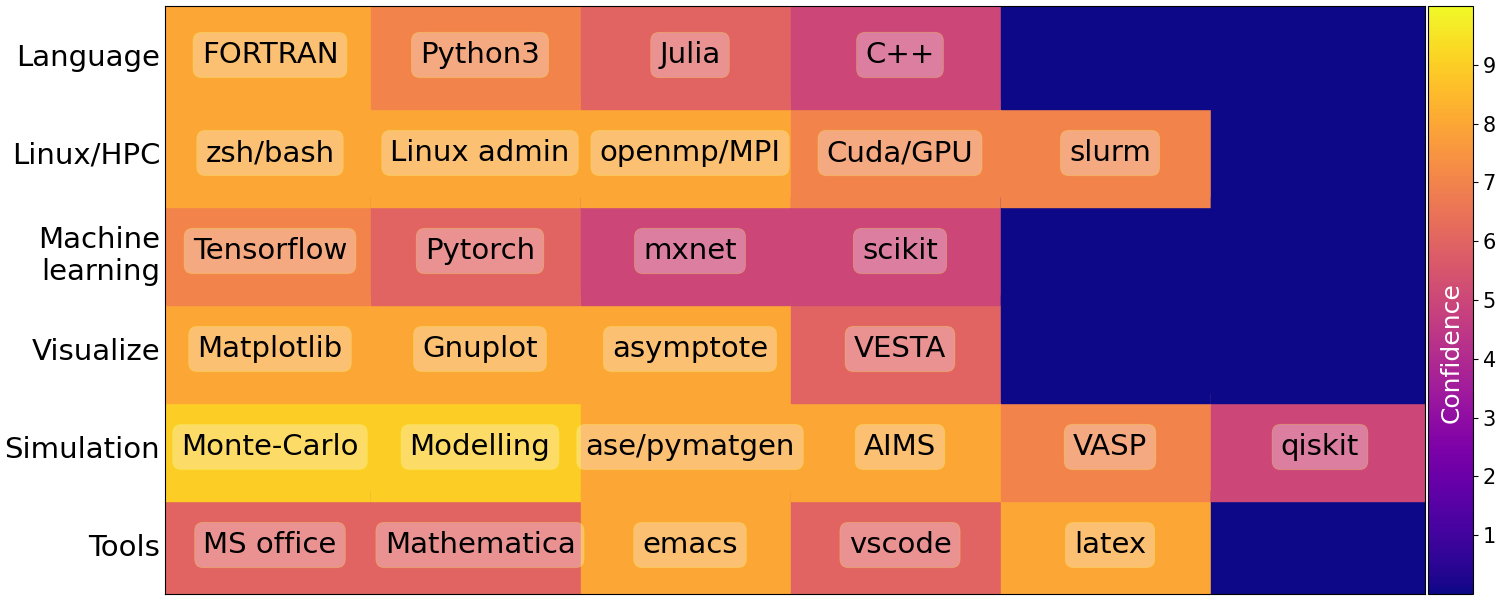
\includegraphics[width=\textwidth]{skills.png}

\vspace{0.9cm}

\section{Research Interests}
%\vspace{0.3cm}
My research insterest include solving models of electron correlation, high throughput \textit{ab-initio} simulations
for material science. I also explore the use of Machine learning in these fields to expand and accelerate my research.
\vspace{0.5cm}
\mysubsection{Correlated Systems, many-body models}
{
  During my Ph.D. my research interest grew around strongly correlated electronic
  systems, where I primarily worked on models of correlation. I love to explore magnetism,
  transport, frustration, disorder and their interplay in correlated electronic systems,
  such as transition metal Oxides, magnetic perovskites, pyrochlore systems.
  The phenomenology of these systems is best explored with suitably simplified models,
  such Hubbard model, Kondo-Lattice Model, Holstein model, Heisenberg model, and their
  variations/combinations depending on whether the relevant degrees of freedom are
  (i) itinerant electrons, (ii) localized spins, or (iii) phonons.
  I explore solving and analysing appropriate models of correlations through real-space
  based techniques like Monte-Carlo methods and Exact-Diagonalization.
}
%\vspace{0.9cm}
\vspace{0.5cm}

\mysubsection{Machine Learning in material science}
{
  After joining Trinity College Dublin, I expanded my research interests over computational
  materials science along with condensed-matter physics, where I explore application of machine
  learning in (i) solving or learning features in correlated systems and (ii) high-throughput \textit{ab initio}
  calculations. I learnt \textit{ab-initio} simulations tools such as VASP/FHI-AIMS to compute energetics
  of real systems, organize and process the data for ML applications. Here at TCD, we are also
  working on developing a \textit{workflow} to combine \textit{ab-initio} and ML tools to build
  up force fields for simulating large, disordered systems. The ICHEC-Flagship project "EuroCC-AF-3"
  has been quite helpful in this direction.
  \vspace{0.5cm}
  
  Following are the categories of ML applications I am involved with varying level of intensity -
  \begin{itemize}
  \item Exploring methods for structure property relations of materials
    with use of High-Throughput \textit{ab initio}.
  \item Applying ML in models of many-body physics, such developing ML based lattice density functional theory for models.
  \item Exploring possibilities of DNNs as generative models for solving many-body problems in correlated systems.
  \end{itemize}
}
\vspace{0.5cm}

\section{Computational interests}
%\vspace{0.5cm}

Ever since I joined my Ph.D. program back in India, computational field always intrigued me.
This meant not only learning the languages and tools to do the required computations, but
also learning how the hardware + software works together. I developed interest in Linux/HPC
tools, by installing and exploring numerous linux distributions ranging from Ubuntu to Archlinux.
I like the opportunity to play with new hardwares whenever possible.
\vspace{0.3cm}
My recent interest was exploring GPUs to accelerate some of our calculations. I secured
"NVIDIA Academic Hardware Grant" last year, and had the GPUs installed in HPC machines,
which boosted the group's interest. As a result, this year half of our group, and others as showed
interests and applied for the same grant for a range of projects.
\vspace{0.3cm}
We are also slowing gearing towards Quantum Computation (QC) in the area where some of our expertise may find
overlap. One of the direction we percieve could be the application of QC in solving many-body problems. However,
my current exposure is limited to some exploration of Qiskit package and a course of IBM-Quantum Fridays.
I am however interested in exploring this further.

\vspace{0.5cm}

\section{Teaching/training/industry}
\begin{itemize}
\item I often co-supervise (i) summer interns (ii) final year project students and (iii) Ph.D. students
  in Prof. Sanvito's group over a range of problems on solving many-body models, \textit{ab-initio} and machine learning.
  Some of the undergrads develop interest in academia and join Ph.D. programme either at Trinity with us or elsewhere.
  \vspace{0.3cm}
\item I have worked in past on projects partnered with Industry as AMBER researcher, such as Nokia's project for
  ``searching corrosion resistant metal alloys'', and recently, modelling magnetism in High Entropy Alloys.
  \vspace{0.3cm}
\item I coordinate with Trinity HPC team for our group's computational requirements. We have developed a local ecosystem
  to facilitate the necessary training, softwares, and other computational needs to younger members of the group.
  \vspace{0.3cm}
\item I also participate in preparing the hardware specifications and tenders of HPC systems/workstations that we purchase.
\end{itemize}

\section{Publications}
%\vspace{0.5cm}
\begin{enumerate}
  
\item
  \textit{Emergence of highly bond-dependent anisotropic magnetic interactions in Sr$_4$RhO$_66$: a theoretical study}
  S.~K.~Pandey, Q.~Gu, R.~Tiwari, arXiv:2207.05045, 2022.
\item %{tiwari2021reac}
  \textit{Reactivity of transition-metal alloys to oxygen and sulfur}, R.~Tiwari, J.~Nelson, C.~Xu, and S.~Sanvito, PRMaterials~\textbf{5} 083801, 2021.

\item %{nelson2021ml}
  \textit{Machine-learning semilocal density functional theory for many-body lattice models at zero and finite temperature},
  J.~Nelson, R.~Tiwari, and S.~Sanvito, PRB~\textbf{103} 245111, 2021.
  
\item %{saket2020orbmott}
  \textit{Orbital mott transition in two dimensional pyrochlore lattice}, A.~Saket and R.~Tiwari, JPCM \textbf{32} 255601, 2020.

\item %{nelson2019ml}
  \textit{Machine learning density functional theory for the hubbard model}, J.~Nelson, R.~Tiwari, and S.~Sanvito, PRB~\textbf{99} 075132, 2019.

\item %{liu2018crdop}
  \textit{Cr doping induced negative transverse magnetoresistance in Cd$_3$As$_2$ thin films}, Y.~Liu \textit{et al}, PRB~\textbf{97} 085303, 2018.
  
\item %{swain2016mottpyro}
  \textit{Mott-hubbard transition and spin-liquid state on the pyrochlore lattice}, N.~Swain, R.~Tiwari, and P.~Majumdar, PRB~\textbf{94} 155119, 2016.
  
\item %{tiwari2014epl}
  \textit{Spectroscopic signatures of the mott transition on the anisotropic triangular lattice}, R.~Tiwari and P.~Majumdar, EPL~\textbf{108} 27007, 2014.
  
\item %{tiwari2013mottfcc}
  \textit{Mott transition and glassiness in the face centered cubic lattice}, R.~Tiwari and P.~Majumdar, arXiv:1302.2922, 2013.

\item %{tiwari2013crossover}
  \textit{The crossover from a bad metal to a frustrated mott insulator}, R.~Tiwari and P.~Majumdar, arXiv:1301.5026, 2013.
  
\item %{tiwari2013noncol}
  \textit{Noncollinear magnetic order in the double perovskites}, R.~Tiwari and P.~Majumdar, IJMP B, \textbf{27} 1350018, 2013.

\item %{tiwari2012visualizing}
  \textit{Visualizing the mott transition}, R.~Tiwari and P.~Majumdar, Current Science \textbf{103} 518-524, 2012.
  
\item %{archer2011exchange}
  \textit{Exchange interactions and magnetic phases of transition metal oxides: Benchmarking advanced ab initio methods}, T.~Archer \textit{et al}, PRB~\textbf{84} 115114, 2011.
\end{enumerate}

\vspace{0.5cm}

\section{References}
\begin{cvcolumns}
  \cvcolumn{Post-Doctoral}{
    Prof. Stefano Sanvito\\ School of Physics and CRANN\\ Trinity College Dublin, Ireland\\\phonesymbol: +35318963065, \\\emailsymbol: sanvitos@tcd.ie
  }
  \cvcolumn{External}{
    Prof. Alessio Filippetti\\ Dipartimento di Fisica, Università di Cagliari, ITALY.
    \\\phonesymbol: (+39) (070) 675 4853, \\\emailsymbol: alessio.filippetti@dsf.unica.it
  }
  \cvcolumn{Doctoral}{
    Prof. Pinaki Majumdar\\ Harish Chandra Research Institute\\ Prayagraj, UP, INDIA\\\phonesymbol: +915322274316, \\\emailsymbol: pinaki@hri.res.in
  }
\end{cvcolumns}


%\newpage
%\section{Cover latter}


\end{document}

%%% Local Variables:
%%% mode: latex
%%% TeX-master: t
%%% End:
